\documentclass[rusmathsym, eqnumwithinsec, amspack, hyperref]{bomgost}

% Закомментируйте это, если hyperref не нужен. 
% Изменение уровня \subparagraph (приложения) в закладках pdf документа. 
% Это нужно для сохранения правильной иерархии закладок в pdf документе.
\makeatletter%
\renewcommand{\toclevel@subparagraph}{2}%
\makeatother% 

% Для вставки программного кода.
\usepackage{listings}

% "Умная" запятая: \(0,2\) - число, \(0, 2\) - перечисление.
\usepackage{icomma}
\usepackage{float}
\usepackage{pgfplots}

\pgfplotsset{compat=newest}

\author{}
\title{Пример на основе класса документа \texttt{bomgost.cls}}
\date{\today}



\begin{document}


\maketitle
\thispagestyle{empty}
\newpage

\begin{abstract}
% Для добавления общего числа приложений нужно добавить команду \printtotapp[.]
% Во всех командах существует необязательный аргумент, который добавляется в конец команды. По умолчанию это запятая. Это нужно для случаев, когда каких-то элементов в работе нет т. е. их счётчики равны 0. В этом случае команда ничего не выведет. Так как порядок команд может быть любым и необходимо, чтобы после последней команды была точка, а между командами запятая, поэтому добавлен необязательный аргумент.
Выпускная квалификационная работа содержит \printtotpage \printtotfig \printtottab \printtotref[.] В~некоторых случаях количество приложений не указывается. 

% Для количества приложений команда аналогична: \total{totappendix}~приложений.

КЛЮЧЕВОЕ СЛОВО~1, КЛЮЧЕВОЕ СЛОВО~2, КЛЮЧЕВОЕ СЛОВО~3 и т. д.

Краткое описание работы.
\end{abstract}


\tableofcontents


\section*{ОБОЗНАЧЕНИЯ И СОКРАЩЕНИЯ}
ОДУ - обыкновенные дифференциальные уравнения.

СЛАУ - система линейных алгебраических уравнений.


\section*{ВВЕДЕНИЕ}
Текст введения.


\mainpart


\section{ТЕОРЕТИЧЕСКАЯ ЧАСТЬ}
\subsection{Первый подраздел}
\subsubsection{Максимальный уровень}
Здесь какой - то текст. Квадратное уравнение.

\begin{equation}
f(x) = x^2 + x-2.
\end{equation}

График представлен на рисунке ниже.
% Важно добавлять каждый рисунок в окружение gostfigure, чтобы был правильный подсчёт общего числа рисунков.
\begin{gostfigure}
\begin{figure}[H]
\centering
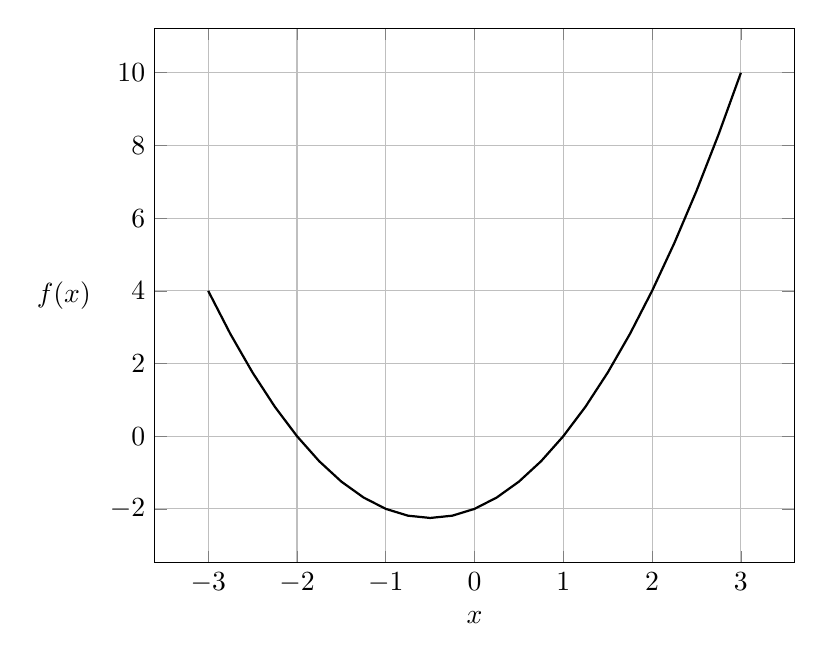
\begin{tikzpicture}
\begin{axis}[domain=-3:3, width = 0.8 \textwidth, grid = both, ylabel style={rotate=-90}, xlabel = \(x\), ylabel = \(f(x)\)]
\addplot[mark=none, thick]{x*x + x - 2};
\end{axis}
\end{tikzpicture}
\caption{График \(f(x)\).}
\end{figure}
\end{gostfigure}

Корни квадратного уравнения представлены в~таблице~\ref{tab:roots}.
% Аналогично с таблицами.
\begin{gosttable}
\begin{table}[H]
\centering
\caption{Корни квадратного уравнения.}
\label{tab:roots}
\begin{tabular}{|c|c|}
\hline 
Первый корень &  Второй корень \\ 
\hline 
1 & -2  \\ 
\hline 
\end{tabular}
\end{table}
\end{gosttable}



\section{ПРАКТИЧЕСКАЯ ЧАСТЬ}
\subsection{Дифференцирование}
\subsubsection{Дифференцирование квадратного уравнения}
\begin{equation}
\dfrac{d f(x)}{d x} = 2 x + 1.
\end{equation}

\section*{ЗАКЛЮЧЕНИЕ}
Интересная стать~\cite{Cybenko}, связанная с~нейронными сетями.

% Список литературы.
\begin{thebibliography}{11}
\bibitem{Bard} Бард Й. Нелинейное оценивание параметров / Й. Бард, Москва: Статистика, 1979. 349 c.
\bibitem{Volterra} Вольтерра В. Математическая теория борьбы за существование // Усп. физ. наук. 1928. № 1 (8). C. 13–34.
\bibitem{Cybenko} Cybenko G. Approximation by Superpositions of a Sigmoidal Function // Mathematics of Control, Signals, and Systems. 1989. (2). C. 303–314.
\end{thebibliography}

\appendix

\begin{gostappendix}{Программный код}
\lstset{language=[11]c++,basicstyle=\ttfamily, showstringspaces=false}

\begin{lstlisting}
#include <iostream>

using namespace std;

int main()
{
  auto b = 1;
  auto a = 2;
  cout << "2 + 1 = " << a + b << endl;
  return 0;
}
\end{lstlisting}
\end{gostappendix}


\begin{gostappendix}{Таблица}
\begin{table}[H]
\centering
\begin{tabular}{|c|c|c|c|}
\hline 
67 & 67 & 7 & 4 \\ 
\hline 
47 & 87 & 71 & 13 \\ 
\hline 
984 & 12 & 354 & 7 \\ 
\hline 
748 & 89 & 2 & 31 \\ 
\hline 
124 & 78 & 99 & 993431 \\ 
\hline 
56 & 12 & 33 & 1554 \\ 
\hline 
48 & 58 & 78 & 12 \\ 
\hline 
102 & 1205 & 1112 & 35 \\ 
\hline 
97 & 888 & 436 & 64 \\ 
\hline 
1 & 2 & 4 & 7 \\
\hline
984 & 12 & 354 & 7 \\ 
\hline 
748 & 89 & 2 & 31 \\ 
\hline 
124 & 78 & 99 & 993431 \\ 
\hline 
56 & 12 & 33 & 1554 \\ 
\hline 
48 & 58 & 78 & 12 \\ 
\hline 
102 & 1205 & 1112 & 35 \\ 
\hline 
97 & 888 & 436 & 64 \\ 
\hline 
1 & 2 & 4 & 7 \\
\hline
748 & 89 & 2 & 31 \\ 
\hline 
124 & 78 & 99 & 993431 \\ 
\hline 
56 & 12 & 33 & 1554 \\ 
\hline 
48 & 58 & 78 & 12 \\ 
\hline 
102 & 1205 & 1112 & 35 \\ 
\hline 
97 & 888 & 436 & 64 \\ 
\hline 
1 & 2 & 4 & 7 \\ 
\hline 
\end{tabular} 
\end{table}
\end{gostappendix}


\end{document}
